% AI506 Data Mining and Search (Spring 2026)
% Term Project Final Report
% Single-file LaTeX report based on the provided ACM template.

\documentclass[sigconf, nonacm]{acmart}
\usepackage{graphicx}
\usepackage{balance}
\usepackage{booktabs}
\usepackage{array}
\usepackage{tikz}
\usetikzlibrary{positioning, arrows.meta, shapes.geometric}
\usepackage{subcaption}
\usepackage{float}
\usepackage{amsmath}
\setlength{\emergencystretch}{3em}
\tolerance=1000
\hbadness=10000

\settopmatter{printacmref=false}
\renewcommand\footnotetextcopyrightpermission[1]{}
\pagestyle{plain}

\begin{document}

\newcommand{\bit}{\begin{itemize}}
\newcommand{\eit}{\end{itemize}}

\title{AI506 Term Project -- Final Report}

\author{Sangjune Kim}
\affiliation{\institution{KAIST}\city{Daejeon}\state{South Korea}}
\author{Gyuchan An}
\affiliation{\institution{KAIST}\city{Daejeon}\state{South Korea}}
\author{Minseo Kang}
\affiliation{\institution{KAIST}\city{Daejeon}\state{South Korea}}

\begin{abstract}
We study advertisement click behavior in a real-world search-log dataset
through two prediction tasks. Task~1 (click prediction) is an extremely
imbalanced binary classification problem (click rate $\approx 1.1\%$) whose
validation set is dominated by cold users; Task~2 (ad prediction) is a
zero-history retrieval problem ranking the clicked ad among $17{,}518$
candidates. For Task~1 we show that the direct text similarity between a
query and a displayed ad barely separates clicks from non-clicks, and we
instead exploit a collaborative signal we call \emph{Semantic K-Nearest-Neighbor
Click Prediction} (SKNCP): we look up the ads that were clicked by the most
similar past queries and measure how similar the current ad is to them. We
empirically validate the smoothness assumption that this signal relies on
(similar queries click on similar ads), and use SKNCP plus trusted
click-through-rate (CTR) features as a small correction to a click-tuned
content score, reaching a clicked-class F1 of $0.1109$ on the
external validation set (bootstrap mean $0.104$, 95\% CI $[0.067,\,0.144]$),
exceeding the provided baseline ($0.0436$) by $+154\%$. For Task~2 we represent queries, ads, and users in a shared text
embedding space and maintain multiple per-user interest vectors updated online;
this reaches NDCG@3 $=0.1538$, improving over a text-similarity-only baseline by
$+55\%$. We choose deterministic Task~1 components (weights, $K$, and threshold)
on an internal split of the training data and report the final external score
using the frozen content-score cache included with the submission files.
\end{abstract}
\maketitle

\section{Introduction}
\label{sec:intro}

Online advertising platforms select advertisements based on search queries,
user context, and ad metadata, and a user's click is a sparse but direct signal
of interest. In this project we study this setting through two related
prediction tasks defined over the same real-world search-log dataset. The two
tasks are formally distinct and require independent submissions; accordingly our
work proceeds along two parallel tracks with task-specific models motivated by
separate exploratory findings.

\subsection{Problem Definition}

\paragraph{Common notation.}
Let $\mathcal{U}$, $\mathcal{S}$, and $\mathcal{A}$ denote the sets of users,
search events, and advertisements. For a search event $s\in\mathcal{S}$, let
$u_s\in\mathcal{U}$ be the issuing user, $x_s\in\mathbb{R}^d$ its
\emph{query embedding}, and for an ad $a\in\mathcal{A}$ let $z_a\in\mathbb{R}^d$
be its \emph{ad-title embedding}, with $d=384$. Embeddings are precomputed with
a pretrained sentence encoder (MiniLM) and are \emph{frozen}. The training log
is a set of displayed-ad impressions
$\{(s_i,u_{s_i},a_i,r_i,h_i,y_i)\}_{i=1}^{N}$ with $N=320{,}000$, where
$r_i$ is the display position, $h_i$ the engine-provided historical CTR, and
$y_i\in\{0,1\}$ the click label. For a search event $s$, we write $a_s^+$ for
its clicked ad (when one exists) and $z_{a_s^+}$ for its embedding; this lets us
distinguish a user's \emph{search intent} $x_s$ from the \emph{clicked-ad
representation} $z_{a_s^+}$, a distinction the Task~2 model relies on.

\paragraph{Terms used throughout.}
\bit
\item \textbf{CTR} (click-through rate): fraction of impressions that are
clicked. The \emph{global} training CTR is $\mu\approx0.0111$.
\item \textbf{HistCTR} $h_{s,a}$: the historical CTR estimate \emph{supplied by
the search engine} for the displayed (ad, position); an input feature.
\item \textbf{Smoothed entity CTR}: for an entity key $g$ (an AdID, IPID,
device, or category), the train-only Laplace-smoothed click rate
$\mathrm{ctr}(g)=\big(\mathrm{clicks}(g)+k\mu\big)/\big(\mathrm{count}(g)+k\big)$
with $k=20$; unseen keys fall back to $\mu$.
\item \textbf{Internal split / external validation.} Model choices
(features, hyper-parameters, decision thresholds) are made on an
\emph{internal} split of the 320k training log: we sort by SearchID and use the
first $80\%$ ($256{,}157$ rows) as internal-train and the last $20\%$
($63{,}843$ rows) as internal-validation. The \emph{external validation} set is
the separately provided \texttt{click\_validation} file ($20{,}000$
impressions); it is held out for final F1/AUC measurement.
\item \textbf{Evaluation.} Task~1 uses clicked-class
$F_1=2\,\mathrm{TP}/(2\,\mathrm{TP}+\mathrm{FP}+\mathrm{FN})$; Task~2 uses
NDCG@3. \emph{AUC} (area under the ROC curve) measures ranking quality
independently of threshold. \emph{Cohen's $d$} denotes a standardized mean
difference (effect size).
\item Task-specific terms are defined formally where first
used, in Sections~\ref{sec:task1} and \ref{sec:task2}.
\eit

\paragraph{Task 1: Click Prediction.}
\bit
\item \textbf{GIVEN:} a displayed-ad impression $(s,a)$ with search-event ID,
ad ID, position $r_{s,a}$, and HistCTR $h_{s,a}$.
\item \textbf{FIND:} a binary prediction $\hat{y}_{s,a}\in\{0,1\}$ of whether $a$
is clicked in $s$.
\item \textbf{TO MAXIMIZE:} clicked-class $F_1$.
\eit

\paragraph{Task 2: Ad Prediction.}
\bit
\item \textbf{GIVEN:} a search event $s$ whose clicked ad is hidden, plus user,
search-context, ad metadata, and the query/ad embeddings.
\item \textbf{FIND:} three distinct ads ranked by likelihood of being the
clicked ad.
\item \textbf{TO MAXIMIZE:} NDCG@3.
\eit
The candidates are the full pool of $17{,}518$ ads.

\subsection{Exploratory Data Analysis Findings}

Table~\ref{tab:eda-summary} collects the statistics that drive our design.

\begin{table}[H]
\centering
\caption{Exploratory statistics motivating the design choices.}
\label{tab:eda-summary}
\small
\setlength{\tabcolsep}{3pt}
\begin{tabular}{@{}>{\raggedright\arraybackslash}p{0.58\columnwidth}>{\raggedleft\arraybackslash}p{0.34\columnwidth}@{}}
\toprule
Quantity & Value \\
\midrule
Training impressions / clicks / CTR & 320{,}000 / 3{,}560 / 1.11\% \\
External validation impressions / clicks / CTR & 20{,}000 / 229 / 1.15\% \\
Train$\,\cap\,$external SearchID overlap & 1 ($\approx$0.01\%) \\
Cold users in click-prediction validation & $\approx$29\% \\
Users / users with zero clicks & 14{,}133 / 83.1\% \\
Ads with zero observed clicks & 87.1\% \\
Click rate at position 1 vs.\ 7 & 1.29\% / 0.71\% \\
Non-logged-in vs.\ logged-in click rate & 1.20\% / 0.99\% \\
Ads per search (1 / 2) & 57\% / 43\% \\
Mean HistCTR, clicked / non-clicked & 0.022 / 0.0095 \\
Task~1 new users / ads in val.-test & 34.4--45.8\% / 9.0--11.7\% \\
Search--ad category match rate & 53.1\% \\
CTR on category match / mismatch & 0.86\% / 1.39\% \\
Task~1 direct query--ad cosine (clicked vs.\ non) & 0.527 / 0.500 ($d\!\approx\!0.11$) \\
Task~2 query--(clicked vs.\ random) ad cosine & 0.55 / 0.25 ($d\!\approx\!1.56$) \\
\bottomrule
\end{tabular}
\end{table}

Three properties matter most. (i) \emph{Clicks are extremely rare} (1.11\%),
so clicked-class F1 is dominated by where the rare positives land at the top of
the ranking, not by overall accuracy; moreover, $83.1\%$ of users and $87.1\%$
of ads have zero observed clicks, limiting pure collaborative filtering.
(ii) \emph{The validation set is a cold, new-session regime}: external SearchIDs
essentially never appear in training ($1$ overlap), $\approx29\%$ of validation
users are unseen, and the validation/test sets introduce many new users and ads
(34.4--45.8\% and 9.0--11.7\%, respectively), so session-memorizing or
user-specific features do not transfer. (iii) \emph{Text
similarity behaves very differently in the two tasks}, and this distinction is
central to our Task~1 design. In Task~2 the relevant comparison is
\emph{clicked ad vs.\ a random ad} for the same query: clicked ads are much more
query-similar than random ones (mean cosine 0.55 vs.\ 0.25, Cohen's
$d\!\approx\!1.56$), so embedding
similarity is a strong retrieval signal. In Task~1 the relevant comparison is
\emph{clicked vs.\ non-clicked among the already-displayed ads}: here the direct
query--ad cosine barely separates the two classes (0.527 vs.\ 0.500, Cohen's
$d\!\approx\!0.11$),
because the displayed ads are already topically plausible. Task~1 therefore
needs a signal beyond direct text similarity, which motivates the collaborative
SKNCP signal in Section~\ref{sec:task1}.

Two additional tabular priors are useful for Task~1. First, HistCTR is the
strongest supplied per-impression signal: clicked impressions have mean HistCTR
$0.022$, compared with $0.0095$ for non-clicked ones. Second, category equality
is not a reliable relevance rule: search and ad categories match in 53.1\% of
training impressions, but the click rate is lower on matching pairs (0.86\%)
than on non-matching pairs (1.39\%), partly because many search contexts have an
unspecified category. We therefore use smoothed category interactions and
trusted CTR priors rather than a naive match indicator.

These observations yield two qualitatively different problems. Task~1 is a
class-imbalanced classification problem over cold entities with at most two ads
per search (so within-search ranking structure is weak). Task~2 is a
zero-history retrieval problem in which the only signal that generalizes is the
shared embedding space. We address them with independent task-specific models.

\section{Task 1: Click Prediction}
\label{sec:task1}

\subsection{Motivation: from failed direct similarity to SKNCP}

A natural idea is to score an impression by the cosine similarity
$\cos(x_s,z_a)$ between the query and ad embeddings. As noted above, this fails
for Task~1: among displayed impressions the clicked and non-clicked classes are
nearly indistinguishable in direct cosine (external Cohen's $d\!\approx\!0.15$, 
AUC $\approx0.52$--$0.54$). The displayed ads are already topically matched to the
query, so direct text similarity says little about which one is clicked.

We therefore reference \emph{what similar users actually clicked}. We define the
\textbf{Semantic K-Nearest-Neighbor Click Prediction} (SKNCP) signal:
\begin{equation}
\mathrm{SKNCP}(s,a)=
\max_{a'\in\mathcal{C}_K(s)} \cos(z_a, z_{a'}),
\label{eq:skncp}
\end{equation}
where $\mathcal{C}_K(s)$ is the set of ads that were \emph{clicked} in the $K$
training search events whose query embeddings are most similar to $x_s$. In
words: ``find the $K$ past searches most like this one, collect the ads those
searches clicked, and measure how similar the current ad is to the closest of
them.''

\paragraph{Empirical justification.}
SKNCP relies on a \emph{smoothness assumption}: \emph{semantically similar
queries click on similar ads}. We validate this directly. Sampling
$\approx30{,}000$ click pairs and binning by query--query similarity, the
average similarity between their clicked ads increases monotonically with query
similarity (Figure~\ref{fig:smoothness}, Pearson $r=0.336$); the reverse
direction (binning by clicked-ad similarity and measuring query similarity)
gives the same effect ($r=0.341$). The query space and the clicked-ad space
thus move together (a joint structure), which is exactly the condition a
$K$-NN approach needs. We then verify that the resulting signal is strong: for
$2{,}000$ clicked samples, the max cosine between the current clicked ad and the
clicked ads of its $K{=}100$ most similar queries averages $0.879$, versus
$0.674$ for random ads (Figure~\ref{fig:knn}a, Cohen's $d=1.27$), and a per-click
paired comparison shows SKNCP exceeding the random baseline for $\approx80\%$ of
clicks (Figure~\ref{fig:knn}b). On its own SKNCP is only modestly stronger than the direct cosine for click
prediction (external Cohen's $d\!\approx\!0.24$ vs.\ $0.15$), consistent with its
weakness as a stand-alone classifier (Section~\ref{sec:task1-results}). Its value
is as a \emph{feature}: combined with the trusted-CTR, position, and rank signals
the log-linear decision score reaches external Cohen's $d\!\approx\!0.61$---roughly
$4\times$ the direct-similarity baseline.

\begin{figure}[t]
\centering
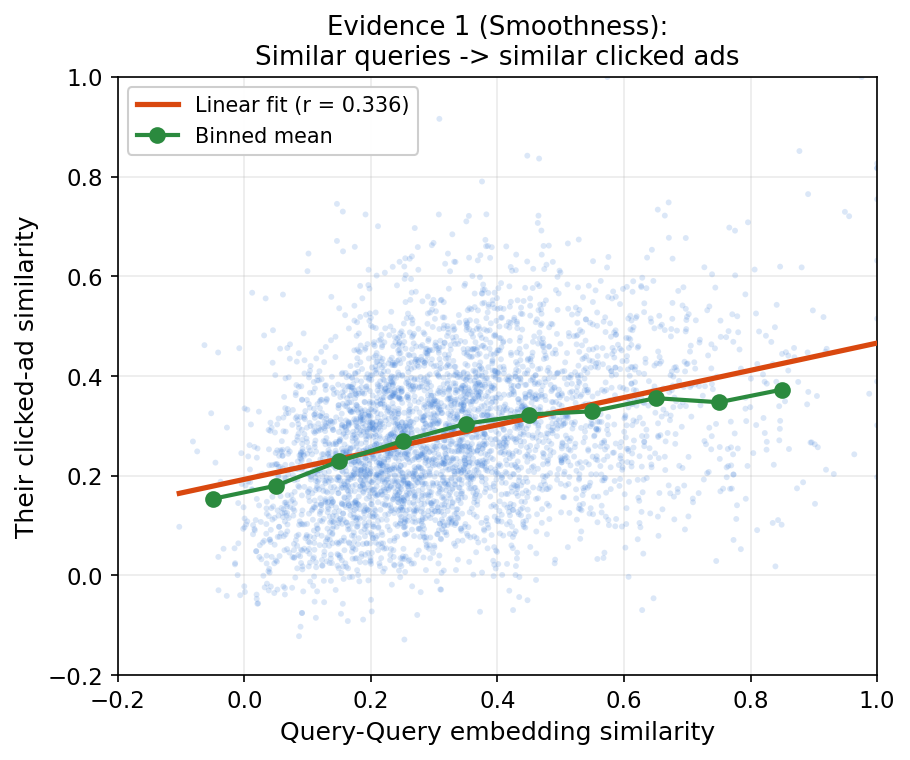
\includegraphics[width=0.82\columnwidth]{evidence_1.png}
\caption{Smoothness assumption (Evidence~1). Each point is a click pair: as the
query--query embedding similarity grows, the similarity between the ads those
queries clicked grows monotonically (binned means and linear fit, $r=0.336$; the
reverse direction gives $r=0.341$).}
\Description{Scatter of click pairs with a positive linear fit of clicked-ad
similarity against query similarity.}
\label{fig:smoothness}
\end{figure}

\begin{figure}[t]
\centering
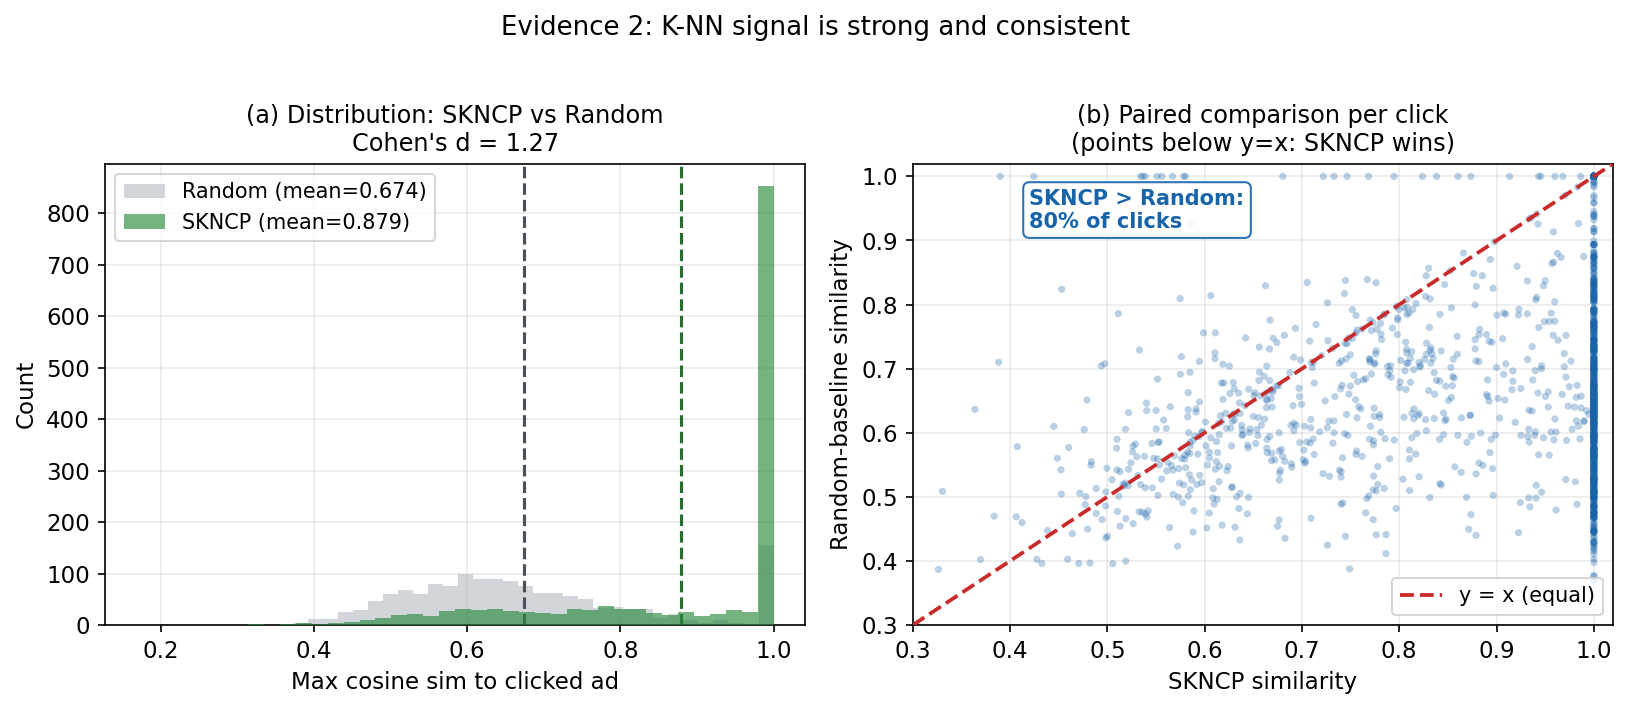
\includegraphics[width=\columnwidth]{evidence_2.png}
\caption{K-NN signal validity (Evidence~2). (a) The current clicked ad is far
more similar to the clicked ads of its similar queries (mean $0.879$) than to
random ads (mean $0.674$), Cohen's $d=1.27$. (b) Per-click paired comparison:
for $\approx80\%$ of clicks the SKNCP similarity exceeds the random baseline.}
\Description{Left: two histograms, SKNCP mean 0.879 vs random mean 0.674. Right:
paired scatter where most points lie on the SKNCP-wins side.}
\label{fig:knn}
\end{figure}

SKNCP alone is nevertheless a \emph{weak} stand-alone classifier
(Section~\ref{sec:task1-results}): its index only contains ads that were
actually clicked in training ($\approx1{,}759$ ads, $\approx67\%$ coverage), so
it cannot score impressions whose neighborhood is empty. We therefore use SKNCP
as a collaborative-filtering \emph{feature} that complements the sparse trusted
CTR signals, not as a model by itself.

\subsection{Methodology}

\paragraph{Signals.}
The auxiliary log-linear component combines signals that are each justified by
the EDA: (1) $\log$ HistCTR, the supplied prior; (2--5) the
$\log$ of smoothed AdID, IPID, device, and category CTRs (defined in
Section~\ref{sec:intro}); (6) an \emph{inverse-propensity-score (IPS) position correction}
$\log(\mathrm{ctr}(\text{pos})/\mu)$ that removes the placement bias measured in
Table~\ref{tab:eda-summary} (position~1 vs.\ 7); (7) the within-search HistCTR
\emph{rank}; (8) SKNCP from Eq.~\eqref{eq:skncp}; and (9) a click-tuned
\emph{content head}. The content head is the cosine of two learned linear
projections of $x_s$ and $z_a$, trained on clicks with a class-balanced
cross-entropy and ensembled over multiple random initializations. Unlike raw
query--ad cosine, this click-tuned text signal is discriminative by itself
(Figure~\ref{fig:content-head}). We then combine the content head with trusted
CTR priors into a cached \emph{content-strong} broad score; this broad score is
the ``content'' term used in the final blend.\footnote{The content head uses
  stochastic training, so re-training it can produce a different content-score
  draw and a slightly different point F1 within the bootstrap confidence
  interval.  To make the submitted result reproducible, the reported point F1
  $0.1109$ uses the frozen pre-computed content-score cache submitted with the
  report (\texttt{code/task1/cs\_cache.npz}, MD5
  \texttt{3dc2105\ldots}).} A fixed multiplicative login term
$\log(1.7)$ is added for non-logged-in rows (EDA: their CTR is higher).

\paragraph{Content-head validation.}
Figure~\ref{fig:content-head} explains why the learned content head is retained
as the broad semantic signal. On the external validation impressions, the pure
content head reaches AUC $0.675$, much stronger than raw query--ad cosine
($\approx0.52$--$0.54$). Its highest score decile has a click rate of $3.3\%$,
nearly three times the base click rate of $1.15\%$. This does not solve the
top-$k$ F1 problem by itself, because clicks are still extremely rare, but it
provides the only dense signal that transfers to cold users and ads. The
content-strong score used in the final blend adds the stable CTR priors to this
head, yielding AUC $0.713$ and F1 $0.106$ before the SKNCP correction.

\begin{figure}[t]
\centering
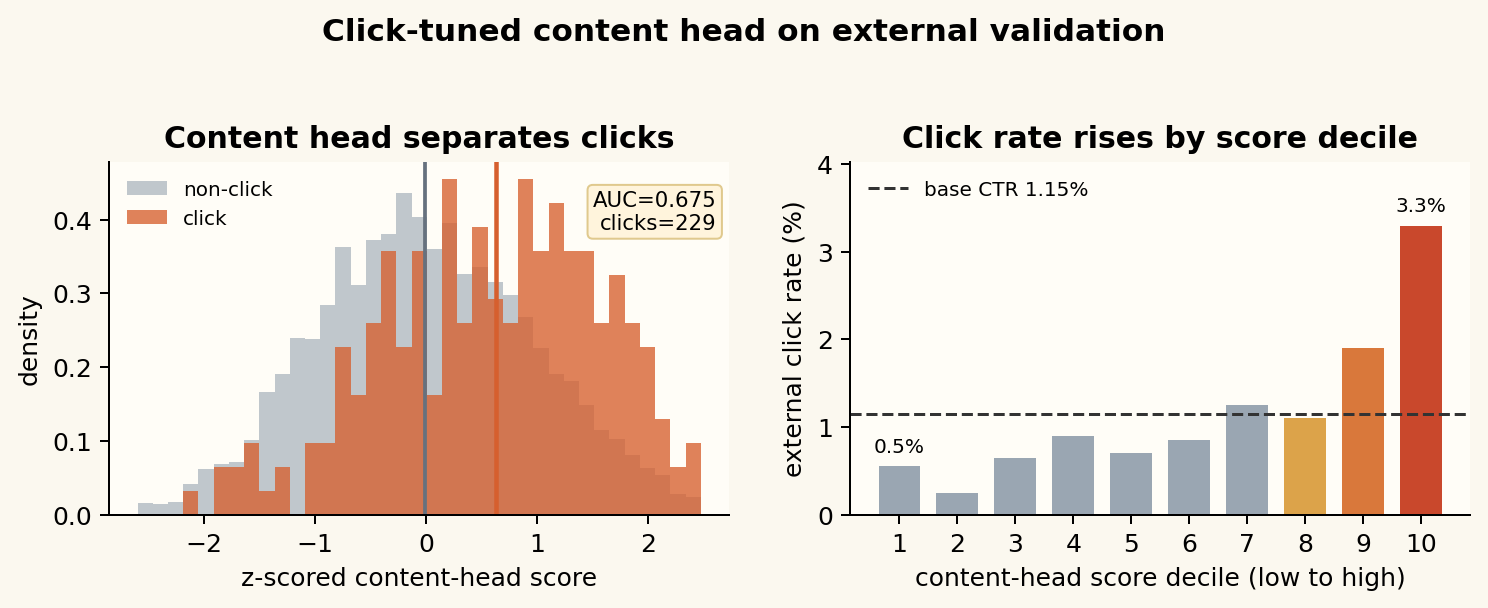
\includegraphics[width=\columnwidth]{content_head_signal.png}
\caption{Click-tuned content-head evidence on external validation. Left: clicked
impressions shift to higher learned content-head scores than non-clicked
impressions (AUC $0.675$). Right: the click rate increases with score decile,
with the top decile reaching $3.3\%$ vs.\ the $1.15\%$ base CTR.}
\Description{Two-panel figure: score distributions for clicked and non-clicked
impressions, and click rate by content-head score decile.}
\label{fig:content-head}
\end{figure}

\paragraph{Fitting.}
We weight the signals to directly maximize clicked-class F1 by
\emph{coordinate ascent}: each weight is swept over a grid while the others are
held fixed, choosing the value that maximizes top-$k$ F1 on the
internal-validation split, cycling until convergence. This optimizes the metric
of interest rather than log-loss, which is dominated by the abundant negatives.
All smoothed CTRs and the SKNCP index are built from internal-train only when
scoring internal-validation, and from the full training log when scoring
external validation, so a row never sees its own label.

\paragraph{Final model: content-strong score with an SKNCP/CTR correction.}
The cached content-strong score is the most stable broad ranking signal, while
SKNCP, CTR, position, and rank are sparse but useful near the top of the ranked
list. We therefore do not let the F1-fitted log-linear model replace the
content-strong score.
Instead, we use it as a small auxiliary correction in standardized ($z$-scored)
space:
\begin{equation}
\mathrm{score}(s,a)= z\!\big(\mathrm{content\text{-}strong}\big) + \alpha\, z\!\big(s_{\mathrm{LL}}\big),
\quad \alpha=0.2,
\label{eq:boost}
\end{equation}
where $s_{\mathrm{LL}}$ (the \emph{log-linear score}) is the F1-fit log-linear
combination of the signals above. Inside this auxiliary score, SKNCP receives
the largest fitted weight ($3.0$), but the auxiliary score is multiplied by
$\alpha{=}0.2$ before being added to the main content-strong score. Thus SKNCP
is used as a top-of-list refinement rather than as the dominant global ranking
signal.
The blend weight $\alpha{=}0.2$ is a
fixed a-priori constant; the neighborhood size $K{=}200$ is selected on the
internal split by the procedure of Section~\ref{sec:task1-kselect} (not tuned on
external labels). Predictions take the top fraction of scores equal to the
training click rate ($1.11\%$); this threshold uses no external labels.
Figure~\ref{fig:task1-pipeline} summarizes the pipeline.

\begin{figure}[t]
\centering
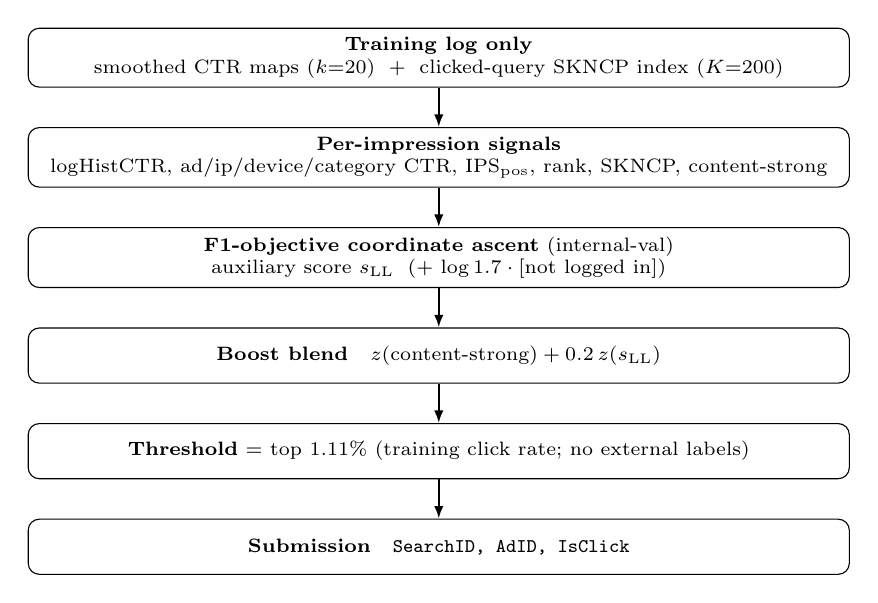
\begin{tikzpicture}[
    node distance=5.0mm,
    box/.style={rectangle, rounded corners, draw=black, align=center,
        minimum width=0.86\columnwidth, minimum height=7mm, font=\scriptsize},
    arrow/.style={-{Latex[length=1.6mm]}, thick}]
\node[box] (idx) {\textbf{Training log only}\\ smoothed CTR maps ($k{=}20$) \;+\; clicked-query SKNCP index ($K{=}200$)};
\node[box, below=of idx] (feat) {\textbf{Per-impression signals}\\ $\log$HistCTR,\ ad/ip/device/category CTR,\ IPS$_{\text{pos}}$,\ rank,\ SKNCP,\ content-strong};
\node[box, below=of feat] (fit) {\textbf{F1-objective coordinate ascent} (internal-val)\\ auxiliary score $s_{\mathrm{LL}}$ \;(+ $\log 1.7\cdot[\text{not logged in}]$)};
\node[box, below=of fit] (blend) {\textbf{Boost blend}\quad $z(\text{content-strong}) + 0.2\, z(s_{\mathrm{LL}})$};
\node[box, below=of blend] (thr) {\textbf{Threshold} = top $1.11\%$ (training click rate; no external labels)};
\node[box, below=of thr] (out) {\textbf{Submission}\quad \texttt{SearchID, AdID, IsClick}};
\draw[arrow](idx)--(feat);\draw[arrow](feat)--(fit);\draw[arrow](fit)--(blend);
\draw[arrow](blend)--(thr);\draw[arrow](thr)--(out);
\end{tikzpicture}
\caption{Final Task~1 pipeline: a frozen content-strong score corrected by a small
F1-optimized auxiliary score built from trusted CTR, position, rank, and SKNCP
signals.}
\Description{Vertical flowchart of the SKNCP-boosted Task 1 pipeline.}
\label{fig:task1-pipeline}
\end{figure}

\subsection{Selecting the neighborhood size \texorpdfstring{$K$}{K}}
\label{sec:task1-kselect}

The SKNCP feature has one hyper-parameter: the neighborhood size $K$, i.e.\ how
many nearest training queries contribute clicked ads to
Eq.~\eqref{eq:skncp}. We select it on the internal split alone, and we select it
by a deliberately chosen criterion: the \emph{internal-validation Cohen's $d$ of
the boosted decision score} (the standardized mean separation between the
clicked and non-clicked classes), maximized over a grid
$K\in\{50,100,\dots,400\}$.

We select $K$ on Cohen's $d$ rather than on top-$k$ F1 because top-$k$ F1 is
computed from integer true-positive counts among only a few hundred positives, so
as a function of $K$ it is a high-variance estimator unsuitable for
hyper-parameter selection. Cohen's $d$ uses full-sample means and spread and
gives a far more stable selection signal. The criterion is fixed before any
external label is read: the external column of Table~\ref{tab:kselect} is the
result of the selected $K$, not an input to choosing it.

\begin{table}[t]
\centering
\caption{Neighborhood-size sweep for the boosted model. Selection uses only the
internal-validation Cohen's $d$ (leftmost numeric column); its argmax is
$K{=}200$. External columns are reported results, not selection inputs. Produced
by \texttt{models/m06\_skncp/experiments/k\_sweep\_eval.py}.}
\label{tab:kselect}
\small
\begin{tabular}{rccc}
\toprule
 & \multicolumn{1}{c}{\textbf{selection}} & \multicolumn{2}{c}{reported (external)} \\
\cmidrule(lr){2-2}\cmidrule(lr){3-4}
$K$ & int-val $d$ & F1 & AUC \\
\midrule
50  & 0.7240 & 0.1020 & 0.7132 \\
100 & 0.7235 & 0.1064 & 0.7131 \\
150 & 0.7235 & 0.1064 & 0.7131 \\
\textbf{200} & \textbf{0.7342} & 0.1109 & 0.7130 \\
250 & 0.7325 & 0.1064 & 0.7133 \\
300 & 0.7235 & 0.1064 & 0.7131 \\
350 & 0.7235 & 0.1064 & 0.7131 \\
400 & 0.7235 & 0.1064 & 0.7131 \\
\bottomrule
\end{tabular}
\end{table}

The internal-validation $d$ is maximized at $K{=}200$ ($d{=}0.7342$), which is
the value used by the final model. Two robustness observations accompany this
choice. First, the criterion is flat: $d$ varies by under $0.012$ across the
entire grid, so $K$ is not a sensitive hyper-parameter and the selection is not
sensitive. Second, every other $K$ yields external F1 ${=}0.1064$, within the
bootstrap confidence interval of the selected operating point
(Section~\ref{sec:task1-results}), so the reported $0.1109$ sits on a stable
plateau rather than a single tuned spike. $K{=}200$ is chosen because it
maximizes the internal $d$; the external F1 of $0.1109$ follows from that choice.

\subsection{Results}
\label{sec:task1-results}

Table~\ref{tab:task1-results} reports external-validation performance. The
deterministic weights, threshold, and SKNCP neighborhood size are chosen on the
internal split; the reported point score uses the submitted frozen content-score
cache. SKNCP alone is weak (F1 $0.027$), confirming it is a complementary
feature rather than a classifier. The content-strong baseline already reaches
F1 $0.106$. The final SKNCP-boosted model attains
$F_1=0.1109$ (AUC $0.713$), a $+154\%$ relative improvement over the provided
baseline ($0.0436$). A $2000$-resample bootstrap gives a mean F1 of $0.104$ with
a wide $95\%$ confidence interval $[0.067,0.144]$.  The interval is wide by
construction: the external set contains only $229$ positives, and the model
predicts $k=222$ clicks with $\mathrm{TP}=25$.  A single true-positive swing
corresponds to $\Delta F_1\!\approx\!0.004$, so the raw variance of the point
estimate is high; differences below $\approx\!0.04$ are within sampling noise.
We therefore report AUC as the more stable ranking metric alongside F1.

\begin{table}[t]
\centering
\caption{Task~1 external validation (clicked-class F1). Threshold = training
click rate ($k{=}222$) unless noted. $^\dagger$Content-strong row uses an
internal-validation positive rate as threshold ($k{\approx}616$); its
precision/recall are not comparable to the other rows.}
\label{tab:task1-results}
\small
\setlength{\tabcolsep}{4pt}
\begin{tabular}{lcccc}
\toprule
Configuration & F1 & Prec. & Recall & AUC \\
\midrule
Provided baseline (HistCTR$>$0.01) & 0.0436 & --- & --- & --- \\
HistCTR only & 0.064 & --- & --- & 0.685 \\
SKNCP only & 0.027 & --- & --- & 0.573 \\
Content-strong baseline$^\dagger$ & 0.106 & 0.073 & 0.196 & 0.713 \\
\textbf{SKNCP-boosted (final)} & \textbf{0.1109} & 0.113 & 0.109 & 0.713 \\
\bottomrule
\end{tabular}
\end{table}

A stratification of the validation users by their training history, computed in
the content-strong analysis before the final SKNCP correction, makes the role of
the semantic component concrete. On \emph{warm} users (with click history,
$21\%$), the model is strongest (F1 $0.12$); on \emph{cold} users (unseen,
$29\%$), the trusted user-specific CTRs are unavailable and the click-tuned
content score carries the prediction (F1 $0.11$). The largest and hardest
stratum is search-history-only users ($49\%$), where ranking quality is high
(AUC $0.73$) but positives are hard to push above the global threshold. This is
the empirical reason the final model needs both a generalizing semantic signal
and the SKNCP/CTR refinement.

\section{Task 2: Ad Prediction}
\label{sec:task2}

\subsection{Motivation and Approach}

The proposed method is motivated by the retrieval nature of Task 2 and the sparsity of explicit click signals in the dataset. In this task, the model must predict which advertisement was clicked for a given search event. Click history provides the most direct evidence of user preference, because a clicked advertisement indicates an explicit positive interaction. However, exploratory analysis shows that click events are sparse for many users, making it difficult to construct reliable personalized representations from clicks alone(among 14,133 users in the training set, 83.1\% of users, or 11,748 users, have no click events). In contrast, search events are more broadly available and each query is represented by a pre-computed text embedding. Therefore, we use search embeddings as an additional behavioral signal to compensate for the sparsity of click history.

For each search event, the query embedding represents the semantic context of the user’s search. This makes query--advertisement semantic compatibility a natural signal for ranking candidate advertisements. However, query-level relevance alone is not sufficient for personalized advertisement prediction. The same or similar queries can be issued by different users with different interests, and these users may click different advertisements under similar search contexts. This suggests that Task 2 requires not only matching advertisements to the given query, but also modeling user-specific preference.

To address this, we represent each user with \textbf{multiple interest} vectors rather than a single global embedding. These vectors are constructed using both search query embeddings and clicked advertisement embeddings. Search queries provide dense but relatively weak behavioral evidence, while clicked advertisements provide sparse but stronger preference evidence. In the update process, clicked advertisements are assigned larger weights than search queries so that explicit positive feedback has a stronger influence on the user representation. This allows the model to build a user-specific multi-interest profile even when click history is limited. 

Based on this motivation, our method ranks candidate advertisements by combining query-level relevance and user-level preference. Query--advertisement similarity captures how well a candidate advertisement matches the given search context, while advertisement--interest similarity captures how well the advertisement matches the user’s learned multi-interest profile. Because queries, advertisements, and user interests are all represented in the same embedding space, the model can perform lightweight ranking using cosine similarity without additional projection layers or complex feature engineering. 

\subsection{Methodology}
\begin{figure}[h]
    \centering
    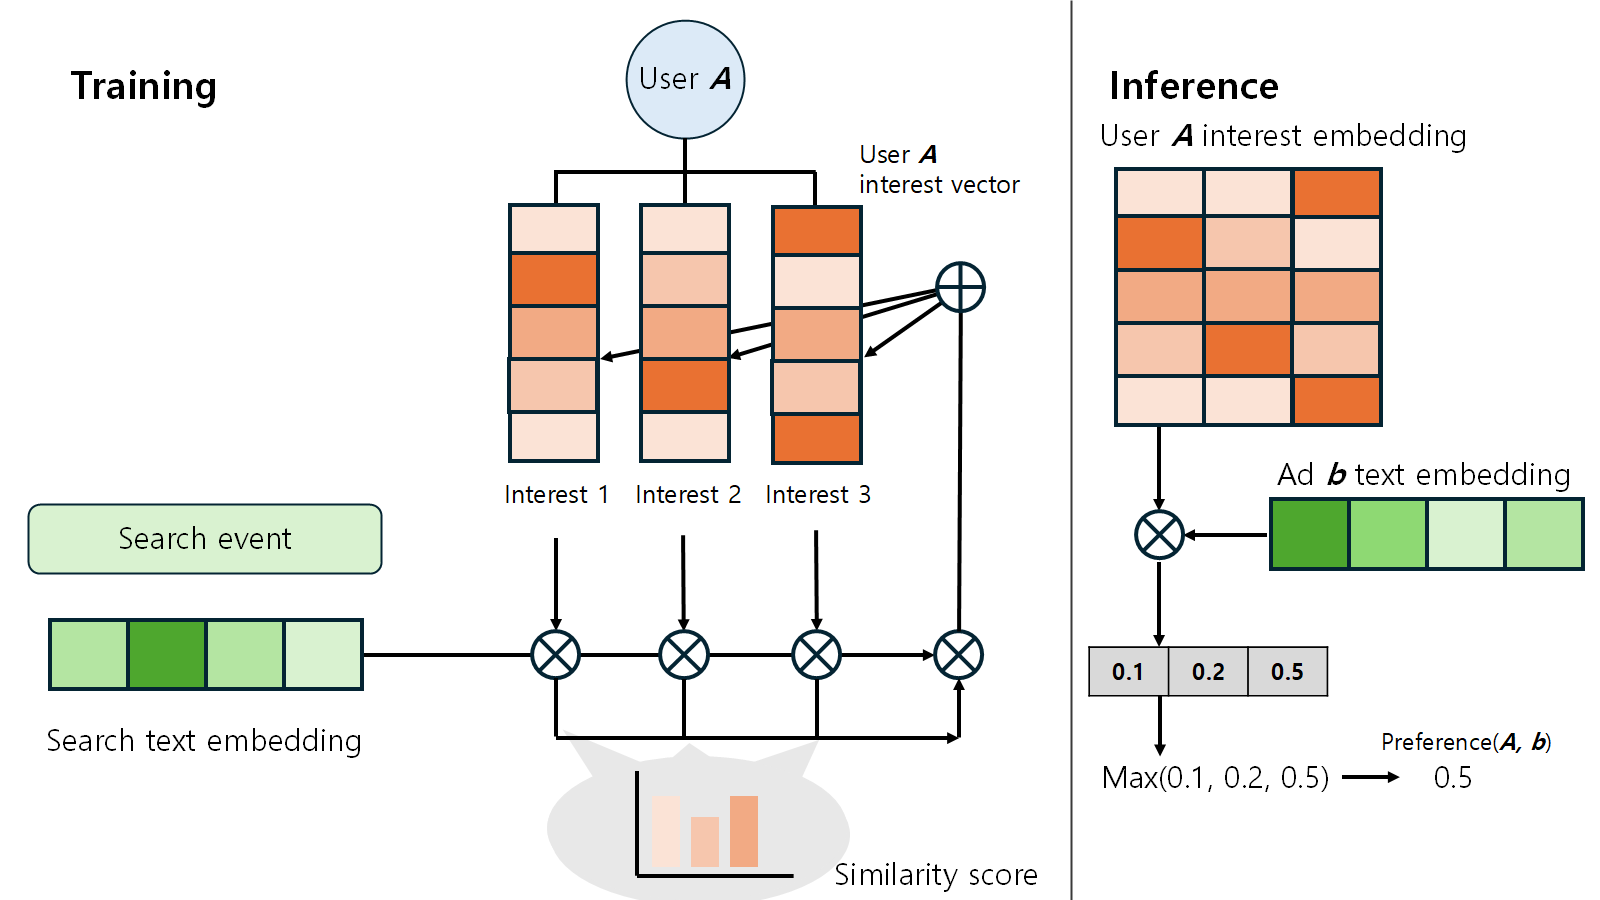
\includegraphics[width=1\linewidth]{figure 1.png}
    \caption{Task~2 multi-interest model architecture.}
    \label{fig:example}
\end{figure}
Our method is a lightweight multi-interest retrieval model that directly uses the provided text embeddings. The main idea is to represent each user with multiple interest vectors and to rank advertisements by combining the current query context with the user’s historical preference.

For each user (u), we maintain (K) interest vectors,

\[
V_u = {v_{u,1}, v_{u,2}, \ldots, v_{u,K}}, \quad v_{u,i} \in \mathbb{R}^d .
\]
When a new behavioral embedding ($e \in \mathbb{R}^d$) is observed for user \(u\), the model updates all interest vectors using a soft-assignment mechanism. The embedding \(e\) can be either a search query embedding $x_s$\ or a clicked advertisement embedding $z_{a_s^+}$. We first compute the cosine similarity between \(e\) and each interest vector:

\[
c_i = \cos(v_{u,i}, e).
\]

The assignment weight of each interest vector is computed by a temperature-scaled softmax:

\[
w_i =
\frac{\exp(c_i / \tau)}
{\sum_{j=1}^{K} \exp(c_j / \tau)} ,
\]


where $\tau$ is the temperature parameter. A smaller $\tau$ makes the update more concentrated on the most similar interest vector, while a larger $\tau$ distributes the update more evenly.

Each interest vector is updated as

\[
v_{u,i}
\leftarrow
\operatorname{norm}
\left(
v_{u,i} + \eta(e) w_i \hat{e}
\right),
\]

where

\[
\hat{e} = \frac{e}{\lVert e \rVert_2}
\]

is the normalized event embedding, and $\operatorname{norm}(\cdot)$ denotes L2 normalization. The update strength $\eta(e)$ depends on the type of behavioral signal:

\[
\eta(e)=
\begin{cases}
\alpha_{\text{search}}, & \text{if } e=x_s, \\
\alpha_{\text{click}}, & \text{if } e=z_{a_s^+}.
\end{cases}
\]

Since search events are dense but weak signals, we use a small $\alpha_{\text{search}}$. In contrast, clicked advertisements are sparse but stronger positive feedback, so we use a larger $\alpha_{\text{click}}$. This allows the model to use search history to reduce click sparsity while still giving stronger influence to explicit click behavior.

For prediction, the model computes two relevance signals for a search event \(s\) and a candidate advertisement \(a\). The first signal measures query-level semantic relevance:

\[
r(s,a) = \cos(x_s, z_a).
\]

The second signal measures user-level preference by comparing the candidate advertisement with the most relevant interest vector of the user $u_s$:

\[
p(u_s,a) =
\max_{1 \le i \le K}
\cos(v_{u_s,i}, z_a).
\]

The final score combines query-level relevance and user-level preference:
\[
\operatorname{score}(s,a)
=
(1-\gamma_{u_s}) r(s,a)
+
\gamma_{u_s} p(u_s,a),
\]
where \(\gamma_{u_s}\) is an adaptive mixing weight determined by the available user history.

We define \(\gamma_{u_s}\) as
\[
\gamma_{u_s} =
\begin{cases}
\gamma_{\text{click}}, & \text{if } u_s \in \mathcal{U}_{\text{click}}, \\
\gamma_{\text{search}}, & \text{if } u_s \notin \mathcal{U}_{\text{click}} \text{ and } u_s \in \mathcal{U}_{\text{search}}, \\
0, & \text{otherwise},
\end{cases}
\]

\begin{table}[h]
\centering
\caption{Adaptive mixing weight used in the scoring function: The actual values used in our experiments are included.}
\label{tab:adaptive-gamma}
\begin{tabular}{lcc}
\toprule
User type & Condition & \(\gamma_{u_s}\) \\
\midrule
Clicked user & \(u_s \in \mathcal{U}_{\text{click}}\) & 0.7 \\
Search-only user & \(u_s \notin \mathcal{U}_{\text{click}},\ u_s \in \mathcal{U}_{\text{search}}\) & 0.5 \\
Cold-start user & otherwise & 0.0 \\
\bottomrule
\end{tabular}
\end{table}


where \(\mathcal{U}_{\text{click}}\) is the set of users with at least one clicked advertisement in the training data, and \(\mathcal{U}_{\text{search}}\) is the set of users with search history. 

If \(\gamma_{u_s}=0\), the user has no available behavioral history, and the model falls back to query-only ranking:
\[
\operatorname{score}(s,a) = r(s,a).
\]

Otherwise, the user-interest score is computed by comparing the candidate advertisement with the most relevant interest vector $p(u_s,a)$ defined above.
Users with click history receive the largest contribution from the learned interest profile, users with only search history receive a moderate contribution, and cold-start users are ranked only by query--advertisement similarity.
For each validation search event we rank all $17{,}518$ candidates and submit the top three:
\[
\operatorname{Top3}_{a \in \mathcal{A}}
\operatorname{score}(s,a).
\]

This formulation keeps all computations in the shared embedding space of search queries, advertisements, and user interests. Therefore, the model can perform efficient ranking using cosine similarity without additional neural projection layers or complex feature engineering.

\subsection{Results}

\paragraph{Setup.}
We train on $320{,}000$ (search, ad, click) triples using the given data order.
Evaluation uses \texttt{ad\_validation}: 214 queries, one ground-truth
ad each, ranked against all $17{,}518$ candidates.

\paragraph{Baselines.}
\begin{itemize}
  \item \textbf{Random}: uniform random score.
  \item \textbf{HistCTR}: rank by historical CTR within category
    (official baseline).
  \item \textbf{Query-only} ($\gamma\!=\!0$): pure query--ad text
    similarity, no user interest.
\end{itemize}

\begin{table}[h]
\centering
\caption{Ad recommendation results (NDCG@3).}
\label{tab:results}
\small
\begin{tabular}{lcc}
\toprule
Method & NDCG@3 & Rank-1 hits \\
\midrule
Random & 0.0008 & 0 \\
HistCTR (baseline) & 0.0211 & 2 \\
Query-only ($\gamma\!=\!0$) & 0.0989 & 14 \\
\textbf{MultiInterest (ours)} & \textbf{0.1538} & \textbf{17} \\
\bottomrule
\end{tabular}
\end{table}

\begin{table}[h]
\centering
\caption{Rank distribution of ground-truth ads ($n\!=\!214$).}
\label{tab:rankdist}
\small
\begin{tabular}{lrc}
\toprule
Rank & Count & NDCG weight \\
\midrule
1       & 17  & 1.000 \\
2       & 6   & 0.631 \\
3       & 2   & 0.500 \\
$> 3$ & 189 & 0.000 \\
\bottomrule
\end{tabular}
\end{table}

The query-only baseline already surpasses HistCTR by $4.7\times$,
confirming that \textbf{text embedding similarity is the dominant
relevance signal} for this task.


To analyze the contribution of each component, we conduct an ablation study on Task 2 using NDCG@3 as the evaluation metric. The full model uses $K=5$, $\alpha_{\text{search}}=0.01$, $\alpha_{\text{click}}=0.5$, $\tau=0.1$, $\gamma_{\text{click}}=0.7$, and $\gamma_{\text{search}}=0.5$.

\begin{table}[h]
\centering
\caption{Ablation study on Task 2.}
\label{tab:ablation}
\begin{tabular}{lcc}
\hline
Model variant & NDCG@3 & Difference \\
\hline
Full model & \textbf{0.1538} & -- \\
w/o interest & 0.0989 & -0.0550 \\
w/o tiered $\gamma$ & 0.1351 & -0.0187 \\
w/o search signal & 0.1415 & -0.0123 \\
w/o click signal & 0.0866 & -0.0673 \\
\hline
\end{tabular}
\end{table}

The ablation results show that user interest modeling is important for Task 2. Removing the interest component reduces NDCG@3 from 0.1538 to 0.0989, which corresponds to the query-only setting. This confirms that the learned user-interest vectors provide additional information beyond query--advertisement similarity.

Among the behavioral signals, the click signal has the largest contribution. When the click update is removed, NDCG@3 drops to 0.0866, which is even lower than the query-only baseline.This suggests that search-only interest vectors can introduce noisy personalization when they are not anchored by explicit click feedback. The search signal also contributes to performance, but its effect is smaller. Removing the search update decreases NDCG@3 from 0.1538 to 0.1415, indicating that search history is useful as a dense auxiliary signal but is weaker than explicit click feedback.

The tiered adaptive mixing weight also improves performance. Without $\gamma_{\text{search}}$, the model cannot effectively use search-only users, and NDCG@3 decreases from 0.1538 to 0.1351. This result supports our design choice of assigning different mixing weights to clicked users, search-only users, and cold-start users.

We also evaluate the effect of the number of interest vectors (K).

\begin{table}[h]
\centering
\caption{Effect of the number of interest vectors.}
\label{tab:kvec}
\begin{tabular}{lcc}
\hline
$K$ & NDCG@3 & Difference \\
\hline
1 & 0.1392 & -0.0146 \\
3 & 0.1392 & -0.0146 \\
5 & \textbf{0.1538} & -- \\
10 & 0.1362 & -0.0176 \\
\hline
\end{tabular}
\end{table}

The best performance is obtained when (K=5). Smaller values such as (K=1) and (K=3) are less effective because they provide limited capacity to represent multiple user interests. However, increasing (K) to 10 also reduces performance, likely because click feedback is sparse and too many interest vectors make specialization more difficult.




\section{Conclusion}
\label{sec:conclusions}

We presented two methodologically independent, EDA-aligned models for the same
advertising search log. For Task~1, the key insight is that direct query--ad
text similarity is uninformative among displayed impressions (external Cohen's
$d\!\approx\!0.15$); SKNCP alone is only modestly stronger ($d\!\approx\!0.24$),
but combined with CTR, position, and rank signals it lifts the decision score to
$d\!\approx\!0.61$---about $4\times$ the direct-similarity baseline; we validated the underlying smoothness assumption
directly and used SKNCP with trusted CTR and position-bias-corrected signals as
a small correction to a click-tuned content score, reaching a clicked-class F1
of $0.1109$ (bootstrap mean $0.104$, 95\% CI $[0.067,\,0.144]$;
$+154\%$ over the provided baseline), with deterministic weights, $K$, and
threshold chosen on an internal split and the frozen content-score cache
included with the submission. For Task~2, representing queries, ads, and users in a shared text
embedding space and maintaining online multi-interest vectors reaches NDCG@3
$=0.1538$, 7.3× improvement over a HistCTR baseline
. Across
both tasks the shared embedding space is the signal that generalizes to the cold,
new-session evaluation regime, but the two tasks exploit it differently: Task~2
uses it directly for retrieval, while Task~1 must route it through the
collaborative SKNCP signal because direct similarity does not separate clicks
among already-displayed ads. The dominant residual limitation is the scarcity of
positive labels ($229$ on the click-prediction validation set), which makes
small F1 differences statistically indistinguishable and motivates reporting AUC
alongside F1.

\bibliographystyle{plain}
\begin{thebibliography}{9}

\bibitem{ke2017lightgbm}
G.~Ke, Q.~Meng, T.~Finley, T.~Wang, W.~Chen, W.~Ma, Q.~Ye, and T.-Y.~Liu.
\newblock LightGBM: A Highly Efficient Gradient Boosting Decision Tree.
\newblock In \textit{NeurIPS}, 2017.

\bibitem{mcmahan2013}
H.~B.~McMahan, G.~Holt, D.~Sculley, M.~Young, D.~Ebner,
J.~Grady, L.~Nie, T.~Phillips, E.~Davydov, D.~Golovin, S.~Chikkerur,
D.~Liu, M.~Wattenberg, A.~M.~Hrafnkelsson, T.~Boulos, and J.~Kubica.
\newblock Ad Click Prediction: A View from the Trenches.
\newblock In \textit{KDD}, 2013.

\bibitem{reimers2019sbert}
N.~Reimers and I.~Gurevych.
\newblock Sentence-BERT: Sentence Embeddings using Siamese
BERT-Networks.
\newblock In \textit{EMNLP-IJCNLP}, 2019.

\end{thebibliography}

\newpage
\appendix
\section{Appendix}

\subsection{Labor Division}

The team performed the following tasks for this final report.

\bit
\item Dataset audit and consolidation of EDA findings
      [Sangjune Kim, Gyuchan An, Minseo Kang].
\item Task~1 model design, feature engineering, and validation[Gyuchan An].
\item Task~2 multi-interest model design, streaming update logic, and
      validation 
      [Sangjune Kim].
\item Report integration, template formatting, and consistency checks
      [Minseo Kang].
\eit

\subsection{Full Disclosure}

\paragraph{Sangjune Kim.}
He is not doing any dissertation, thesis, or external project related to this 
class project.

\paragraph{Gyuchan An.}
He is not doing any dissertation, thesis, or external project related to this 
class project.

\paragraph{Minseo Kang.}
He is not doing any dissertation, thesis, or external project related to this 
class project.

\paragraph{Use of LLM assistance.}
Large language models, including ChatGPT and Claude, were used for LaTeX editing, wording refinement, and organization
of experimental findings.  The experiments, numerical results, modeling
decisions, and final submissions were produced and verified by the
team.

\end{document}